%-------------------------------------------------------------------------------
\section{Introduction}
\label{s:intro}
%-------------------------------------------------------------------------------

Many microservices are \textit{latency critical} (LC), meaning they are required
to meet strict Service Level Objectives (SLOs), that guarantee uptime and caps
on the response latency of the service. In order to meet these guarantees,
developers reserve resources on cloud systems like AWS ec2 or Kubernetes, where
the reservation interface consists of a fixed amount of resources the service
will get, \ie{} a number of CPUs and an amount of
memory~\cite{aws-ec2-resources, kubernetes-resources}. However, the load on the
microservices is usually variable and unpredictable. Developers choose the
amount of resources to reserve based on the expected peak load, and as a result
the resources are rarely fully used~\cite{borg, nu, overprovision}.

Other tasks do not fall into this category: \textit{best effort} (BE) tasks such
as long-running map reduce jobs or background data analytics do not have an SLO.

Splitting workloads into LC and BE is popular because it allows providers to run
BE tasks on machines reserved for LC tasks that are currently experiencing low
load and thus have idle resources~\cite{perfiso}. Indeed, many cloud scheduling
systems support LC and BE tasks. This includes distributed schedulers, \eg{}
Borg\cite{borg} or Kubernetes\cite{kubernetes-resources}, and single machine
schedulers, for example Caladan\cite{caladan}.

However, enforcing strict isolation is challenging: Should an LC service
experience a spike in load, it needs to be able to immediately have access to
all the resources it had reserved. Any delay likely leads to violations of the
services SLOs.

\begin{figure}[t]
    \centering
    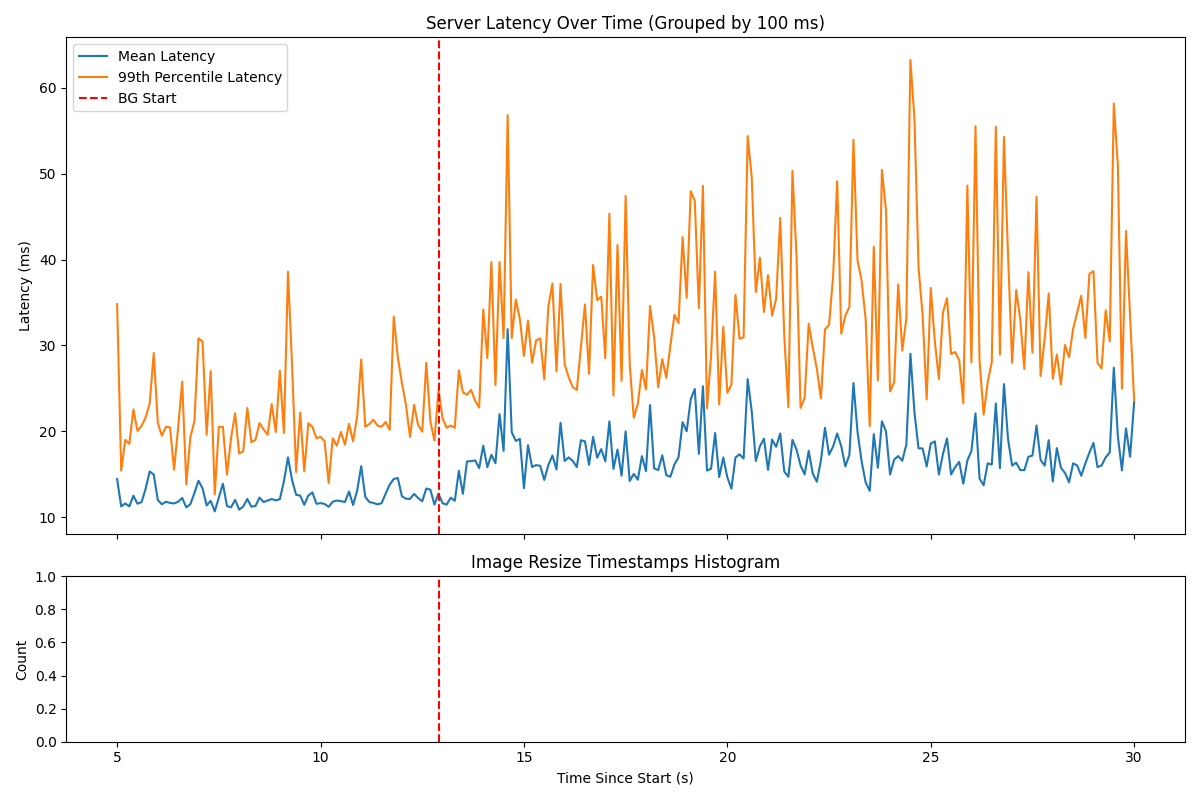
\includegraphics[width=\columnwidth]{graphs/kubernetes-unedited.png}
    \caption{E2E repsonse times for a simple social network web application,
    before and after starting load on a BE
    service}\label{fig:kubernetes-unedited}
\end{figure}

Current popular systems fail to properly isolate latency critical from best
effort workloads. When running a small but realistic social network web
application on Kubernetes, we observe significant impacts on its latency when
starting a best effort workload, doing image resizing, on the same machine. The
top graph of \autoref{fig:kubernetes-unedited} plots the end-to-end latency of
an endpoint that gets a users feed and applies a moderation; the bottom graph
shows the throughput of the BE workload. After the BEs start running, the mean
response latency of the web application jumps from $\sim$7ms to $\sim$15ms, and
the 99th percentile latency from $\sim$10ms to $\sim$23ms . 

Understanding where the isolation fails requires looking at the underlying
mechanism that is enforcing it: Linux's \cgroups{}. \cgroups{} offers an API to
enforce isolation of multiple resources including memory and CPU; this work
focuses on CPU isolation. Most modern containers rely on \cgroups{} for CPU
isolation; this includes all Open Container Initiative (OCI) compliant
containers, including Kubernetes but also Docker, CRI-O, and
containerd~\cite{oci-cgroups,docker-docs-cgroups,container-isolation-article}.
VM frameworks, including Firecracker, AFaas and libvirt, also rely on \cgroups{}
to manage CPU time allocation when the number of vCPUs is
oversubscribed.~\cite{firecracker-cgroups,afaas,libvirt-cgroups}

The part of the \cgroups{} interface that these systems use to isolate LC and BE
is based on weight: each workload is put into its own group, and each group is
assigned a weight in the range [1, 10000]. \cgroups{} specifies that each group
gets CPU time proportional to its weight as a share of the sum of weights of
runnable groups~\cite{cgroups-kerneldocs}.\footnote{Other operating systems use
a similar interface, for instance Windows exposes a number of shares.} For
instance, if two groups $cg1$ and $cg2$ have weights 200 and 300 respectively,
when they are both active their CPU time ratio should also be $2:3$, but if
$cg1$ has no runnable threads, then $cg2$ would represent 100\% of the runnable
weight and get all the CPU time.

However, in \autoref{fig:kubernetes-unedited} the effect the BE has on the
latency of the LC server is much higher than expected for starting a process
with $1/10000$th of the LCs weight. As we show in more detail in
\autoref{s:problem}, the problem that leads to the increased latencies observed
is that Linux will run a BE process on one core, unaware that an LC process is
runnable and waiting on another. This happens because Linux uses per-CPU
runqueues, which avoids the overheads of having a global runqueue. A key
challenge this work addresses is how to manage this tension between expensive
cross-core checks and affecting strict isolation across cores.

Our approach addresses this challenge by exposing in the API and enforcing in
the scheduler a new priority class for BE to run in, \beclass{}. As we show in
\autoref{ss:approach:solves-problems}, putting BE in a separate class from LC
makes it viable to enforce the isolation across cores, because it reduces the
number of times the scheduler is required to look at other runqueues. Enforcing
weights across cores requires the scheduler to do so every scheduling tick, but
with a separate class it only has to look at other cores on \textit{class
boundary crossings}: every time a core starts running a BE process, and every
time it queues an LC one.

A challenge that emerges from creating a separate priority class is that, when
the LC is under high load, the BE processes need somewhere to go. The goal is to
make the priority of LC over BE as strict as possible, while allowing the BE
processes to resume execution once the load has gone down, even if that takes a
couple minutes.

We address this challenge by enabling BEs to exist in an ephemeral state called
\textit{parked}, which BEs are put in when the CPU utilization is high enough
that any amount of running a BE would interfere with an LC. While load remains
high, the scheduler ensures that the user-space process doesn't run and consume
resources, but continues to run the kernel-space handlers that manage critical
state such as TCP connections and timers on behalf of the BE processes. 

We implement \beclass{} in Linux, and show that it is able to significiantly
improve Linux's ability to isolate LC from BE workloads: in the same Kubernetes
experiment, the increase in average latency when starting a BE workload goes
from $>$2x to 0. The contributions of this paper are thus as follows: 
\begin{enumerate}
    \item identifying that the reason isolation of LC from BE often fails is that
    \cgroups{} does a poor job of enforcing the weights of different groups
    across cores; and that this dramatically affects end-to-end latencies
    \item the design of \beclass{}, a new class for BE tasks that separates
    them from the default class LC tasks run in, and isolates LC workloads from
    BE ones while minimizing the amount of cross-core checks required, as well as
    naturally enforcing the parked state
    \item an implementation of \beclass{} in Linux
\end{enumerate}
